Để các thành viên trong nhóm có thể cùng nhau xây dựng hệ thống này một cách hiệu quả nhất, nhu cầu tất yếu phải có một hệ thống quản lý mã nguồn. Nhóm sử dụng \textbf{Git}, một hệ thống quản lý phiên bản phổ biến nhất hiện nay. \textbf{Git} giúp việc cộng tác dễ dàng hơn, cho phép thay đổi của các thành viên được hợp nhất thành một mã nguồn duy nhất.\par

Nhóm chọn sử dụng \textbf{Github}, một nền tảng lưu trữ mã nguồn của Git. Tất cả mã nguồn của Luận văn tốt nghiệp được lưu trữ trên \textbf{Github}.

Đây là đường dẫn dẫn đến trang github quản lý mã nguồn của nhóm:\\ \href{https://github.com/lvtn202}{[https://github.com/lvtn202]}

Phần tiếp theo đây, nhóm sẽ trình bày về cấu trúc của mã nguồn mà nhóm đã hiện thực. Với cấu trúc mà nhóm đã hiện thực, có thể dễ dàng thêm mới các chức năng mà không cần phải thay đổi cấu trúc gốc của dự án.

\textbf{Về phía front-end}

\begin{figure}[H]
    \begin{center}
        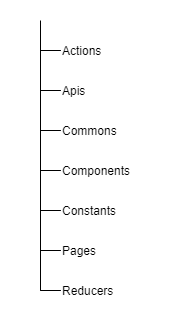
\includegraphics[width=4cm]{Image/Technical/frontend_structure.png}
        \caption{Cấu trúc mã nguồn Front-end}
        \label{frontend_structure}
    \end{center}
\end{figure}

\begin{itemize}
    \item Actions: nơi chứa các hàm nhận sự kiện tương tác của người dùng lên hệ thống, nhiệm vụ của những hàm này là phân biệt sự kiện và chuyển đến reducer tương ứng để thực hiện các chức năng như tính toán, gọi api,...
    \item Apis: nơi chứa khai báo các đường dẫn api để thực hiện request tới backend.
    \item Common: chứa các hàm hỗ trợ thông dụng, có thể sử dụng trong toàn ứng dụng như: xử lí các lỗi api, các hàm định dạng ngày tháng và tiền,...
    \item Components: chứa các giao diện thông dụng như giao diện cảnh báo lỗi, giao diện báo thành công, giao diện loading,...
    \item Contants: chứa các hằng số về loại actions của người dùng, các hằng số được định nghĩa trong dữ liệu của backend,...
    \item Pages: chứa các trang giao diện chính của hệ thống.
    \item Reducers: chứa các reducers của các chức năng, nơi nhận thông báo từ action và thực hiện tính toán.
\end{itemize}





\textbf{Về phía back-end}